\section{High level system overview}
This section addresses high level system design especially.
\begin{itemize}
    \item data structure and data flow
    \item sequential interaction between the system subcomponents
\end{itemize}

\subsection{Data structure and data flow}
We assume that the IMU will provide the following data:
\begin{itemize}
    \item $a_x$ acceleration on the x-axis
    \item $a_y$ acceleration on the y-axis
    \item $a_z$ acceleration on the z -axis
    \item $\omega_x$ angular rate along its x-axis
    \item $\omega_y$ angular rate along its y-axis
    \item $\omega_z$ angular rate along its z-axis
    \item $T$ temperature of the sensor.
\end{itemize}
We assume that the physical sampling of all those values are made at the exact same time, respectively the difference between the sampling time is negligible.
In other word we can timestamp the measurment time with a single timestamp $t_{mes}$.

\subsection{Sequential interaction}
The system has following subsystem:
\begin{itemize}
    \item the IMU itself.
    \item the UART peripheral of the compute platform.
    \item the Operation system Kernel.
    \item the device file that will be created by the kernel to describe the device.
    \item the IMU driver software component.
    \item the IMU message queue.
    \item the Odometry application that will consume the IMU data.
\end{itemize}

\begin{figure}[H]
    \centering
    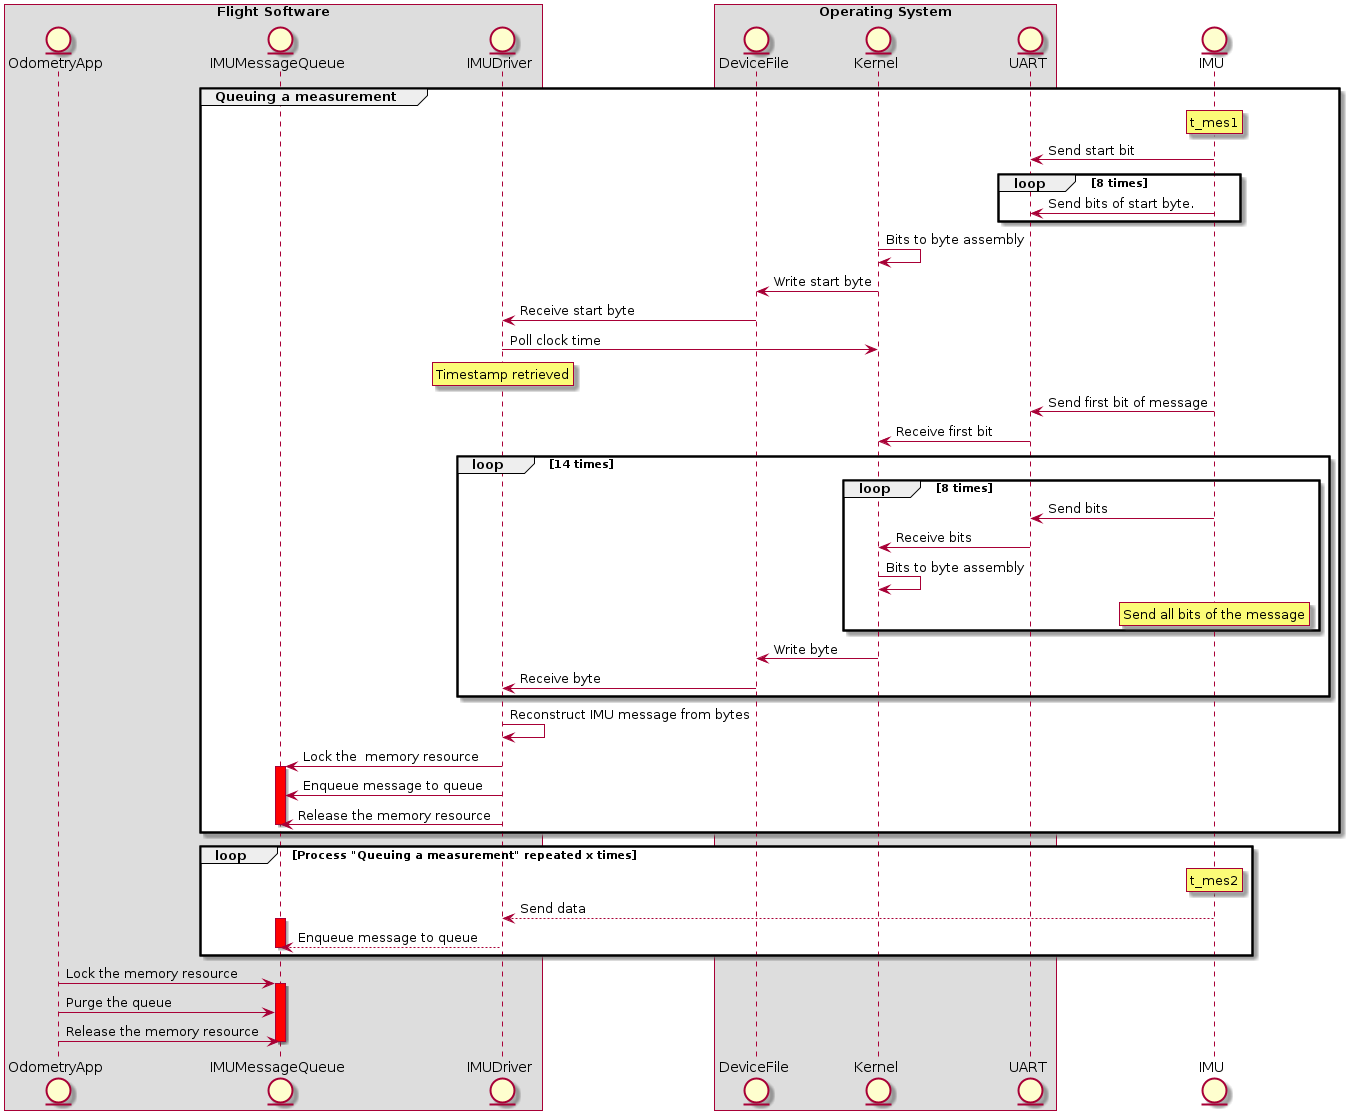
\includegraphics[width=1.0 \textwidth]{diagrams/high_level_sys_overview.png}
    \caption{High level sequence diagram of the nominal operation case}
    \label{fig-high-level-nominal}
\end{figure}

In nominal operation the sequence of intercation (Fig.\ref{fig-high-level-nominal}) is as follow:\\
The IMU make a new measurment at $t_{mes1}$.
It then sends the data for this measurments bit by bit to the UART peripheral.
When the first 8 bits have been received, the low level UART driver of the kernel will write a byte to the device file.
The IMU driver will then poll the clock time and use it to timestamp the measurement.
The rest of the byte are collected and then reconstructed into an IMU message.\\

This process is repeated several times until the OdometryApp purge all message stored in the queue.\\

\subsection{Fault-tree analysis}

\begin{figure}[H]
    \centering
    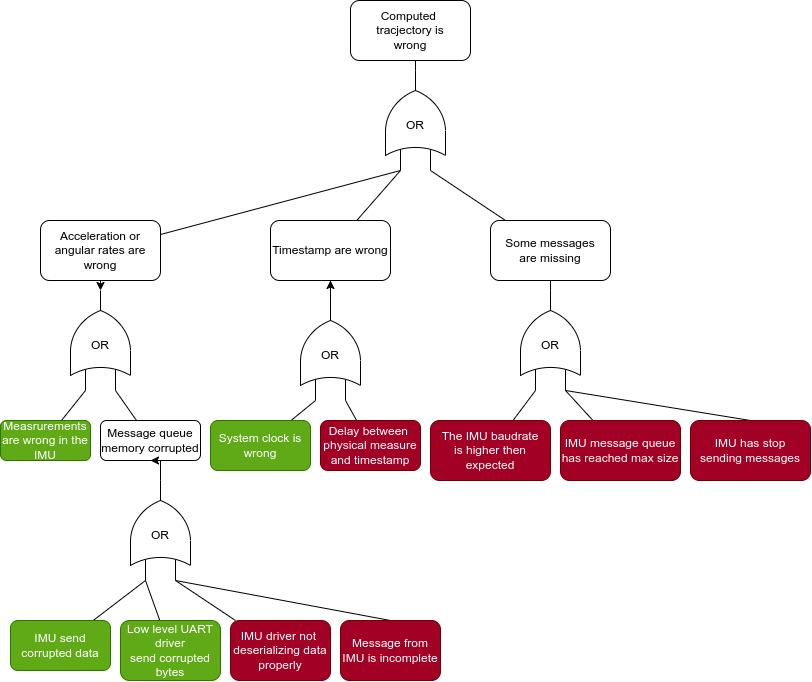
\includegraphics[width=1.0 \textwidth]{diagrams/main_fault_tree.drawio.png}
    \caption{Main fault tree}
    \label{fig-main-fault-tree}
\end{figure}


\subsection{Interface definition}
